\thispagestyle{empty}
\renewcommand*\contentsname{\begin{center}ЗМІСТ\end{center}}
\tableofcontents

%-----------------------------------%

\newpage
\thispagestyle{empty}
\phantomsection
\addcontentsline{toc}{section}{ПЕРЕЛІК УМОВНИХ ПОЗНАЧЕНЬ, СКОРОЧЕНЬ І ТЕРМІНІВ}
%term%
\begin{center}
\textbf{\Large ПЕРЕЛІК УМОВНИХ ПОЗНАЧЕНЬ, СКОРОЧЕНЬ І ТЕРМІНІВ}
\end{center}

\hypertarget{term0}{Трібанк} - https://en.wikipedia.org/wiki/Treebank
\hypertarget{term1}{Крос-платформенна мова програмування}
\hypertarget{term2}{Парсинг}
\hypertarget{term3}{.conllu}
\hypertarget{term4}{UD} - Universal Dependencies
\hypertarget{term5}{Фреймворк} -  інфраструктура програмних рішень, що полегшує розробку 
складних систем https://uk.wikipedia.org/wiki/Програмний\_каркас

%-----------------------------------%

\newpage
\thispagestyle{empty}
\phantomsection
\addcontentsline{toc}{section}{ВСТУП}

\begin{center}
\textbf{\Large ВСТУП}
\end{center}

%-----------------------------------%

\newpage

\section{КОРПУСИ ТЕКСТІВ UNIVERSAL DEPENDENCIES}

% https://applied-language-technology.mooc.fi/html/notebooks/part_iii/02_universal_dependencies.html

\subsection{Обробка природної мови}

\subsection{Проблематика створення фреймворку для розмічення різних мов}

укр - 122275 токенів 122324 слова 7060 реченнь

Корпуси текстів Universal Dependencies або скорочено UD — це проект спільної розробки
з відкритим кодом, який має дві основні цілі:

\begin{enumerate}
    \item розробити загальну структуру для опису граматичної структури різноманітних мов.
    \cite{bib1}
    \item створювати анотовані корпуси або \hyperlink{term0}{трібанки} для різних мов,
    які застосовують цю структуру. \cite{bib2}
\end{enumerate}

Таким чином, проект має на меті забезпечити систематичний опис синтаксичних структур і
морфологічних особливостей у різних мовах, що, у свою чергу, дозволяє проводити порівняння
між мовами.

Лінгвістичні корпуси, які містять анотації для синтаксичних відносин,
часто називають банками дерев (трібанками), оскільки синтаксичні структури, як правило,
представлені за допомогою деревоподібних структур. Таким чином, у цьому контексті трібанк —
це просто набір синтаксичних дерев, які були послідовно анотовані за допомогою UD
або якоїсь іншої структури.

Структура UD є компромісом між кількома взаємопов'язаними критеріями, які наведені нижче:

\begin{enumerate}
    \item UD має бути придатним для комп'ютерного розбору з високою точністю
    \item UD має бути задовільним для лінгвістичного аналізу окремих мов
    \item UD повинен гарно виявляти структурні подібності між спорідненими мовами
    \item UD має бути придатним для швидкого, послідовного анотування людиною-анотатором
    \item UD має бути легко зрозумілим і використаним користувачами, які не знають мови
\end{enumerate}

\subsection{Репозиторій корпусу текстів Universal Dependencies українською}
Як об'єкт для дослідження використовувася \cite{bib3}

\subsection{Формат даних CoNLL-U}

\begin{table}[h]
\begin{tabular}{|l|l|}
\hline
  Field   & Description \\ \hline
ID        & Index of the word in sequence \\ \hline
FORM      & The form of a word or punctuation symbol \\ \hline
LEMMA     & Lemma or the base form of a word \\ \hline
UPOS      & Universal part-of-speech tag \\ \hline
XPOS      & Language-specific part-of-speech tag \\ \hline
FEATS     & Morphological features \\ \hline
HEAD      & Syntactic head of the current word \\ \hline
DEPREL    & Universal dependency relation to the \\ \hline
DEPS      & Enhanced dependency relations \\ \hline
MISC      & Any additional annotations \\ \hline
\end{tabular}
\caption{Table to test captions and labels.}
\label{table:1}
\end{table}


%-----------------------------------%


\section{ЗБІР ДАНИХ І ТОКЕНІЗАЦІЯ} % todo probably rename


%-----------------------------------%


\section{АНАЛІЗ ЗІБРАНИХ ДАНИХ}


%-----------------------------------%


\section{ЗАСОБИ РОЗРОБКИ}

Галузь інформаційних технологій рушила далеко вперед за останні декілька десятків років.
У тому числі в питанні засобів розробки. 


Зараз існує багато інструментів, які покликані
полегшити та покращити досвід написання коду та усі цикли розробки програмного забезпечення
в цілому. З'явилося чимало мов програмування загального призначення,
які все ж зайняли свої певні ніші й використовуються переважно в якійсь одній галузі,
незважаючи на своє загальне призначення. Оскільки ресурси розробників цих мов не необмежені,
вони фокусуються на конкретних функціях та особливостях і реалізовують саме їх. Таким чином,
навіть мови загального призначення відрізняються одна від одної і підходять краще під ті,
чи інші задачі. Тому дуже важливо не бездумно користуватися найпростішим, чи тим інструментом,
який ти знаєш краще, а обирати і вивчати ті, які найкраще підходять під поставлену задачу.

\subsection{Мова програмування Python}

\begin{wrapfigure}{r}{0.3\linewidth}
  \begin{center}
    
\includegraphics[width=\linewidth]{python.png}
  \end{center}
  \caption{Логотип мови Python}
\end{wrapfigure}

Для написання цієї роботи використовувалася мова програмування Python. Це інтерпретована
об'єктно-орієнтована мова програмування високого рівня зі строгою динамічною типізацією.
Ця мова відома, перш за все, за свою відносну простоту та низький поріг входу,
а також за високий темп розробки, внаслідок свого динамічного та інтерпритованого характеру.
Оскільки ця мова інтерпритується віртуальною машиною, а не компілюється під конкретну
операційну систему, це робить її також \hyperlink{term1}{крос-платформенною}.
Але основна причина чому мова Python чудово підходить для задач обробки природної мови
та статистичного аналізу - це велика спільнота науковців та розробників, які створили чималу
кількість бібліотек та інструментів які підвищують рівень абстракції і дозволяють сфокусуватися
на предметі дослідження і не відволікатися на низькорівневі речі, як-от
\hyperlink{term2}{парсинг} вихідних файлів.

\subsubsection{Фреймворк для тестування Unittest}

\subsubsection{Пакетний менеджер Pip}
щось про піп

\subsubsection{Інтегроване середовище розробки PyCharm}
Як основне середовище розробки використовувався рушій PyCharm, 
розроблений компанією JetBrains

\subsection{Система контролю версій Git}
Система Git без сумніву є одним із найголовніших засобів розробки 21 століття. Проблема
керування версіями виникла ще за часів написання перших програм. І загострилася із
експоненційним ростом складності програмного забезпечення.

Системи контролю версій зберігають історію зміни файлу або набору файлів для того,
щоб у майбутньому була змога
повернутися до певної збереженої версії. Системи контролю версій гарантують можливість
відновити втрачені чи пошкоджені файли і легеко повернути їх у робочий стан. Найпростіше
рішення контролю за версіями - це звичайне копіювання файлів у іншу директорію. Це, мабуть,
є найрозповсюдженішим способом вирішення цієї проблеми, внаслідок своєї простоти.
Але у такого способа є фатальні недоліки. По-перше, дуже просто заплутатися у створених
директоріях. По-друге, файли досі зберігаються на локальному носії, що у разі
несправності призведе до втрати усіх файлів. По-третє, такий підхід зовсім 
не масштабується. Із розростанням кодової бази і складності програмного продукту кількість
файлів та директорій буде на стільки великою, що тільки на копіювання буде витрачатися
величезна кількість часу, не кажучи вже про управління і підтримку такої системи.
Тому очевидно що такий підхід непрактичний і нежиттєздатний для розробки програмного
забезпечення.

На заміну такого підходу прийшли системи контролю версій. Перші з них мали звичайну
базу даних, у якій зберігалася інформація про зміну файлів. Однак вони все ще не
вирішували проблему втрати файлів у разі несправності носія. Розподілені системи
по типу Git покликані вирішити і цю проблему. Основною ідеєю таких систем є те, що
усі дані зберігаються не в одному місці (на локальному носії, чи то на віддаленому
сервері), а копіюються на пристрої кожного розробника, що дає змогу відновити усю історію
змін.

Система Git має багато переваг над конкурентами. Завдяки своєму унікальному підходу
до зберігання інформації про зміни файлів, вона може запропонувати такі функції,
які не доступні багатьом конкурентам внаслідок обмеженості їх архітектури.
На відміну від більшості систем, Git зберігає знімки станів кожного з файлів, а не історію
зміни, рис. \ref{img:git_snapshots}.

\begin{figure}[h]
  \begin{center}
    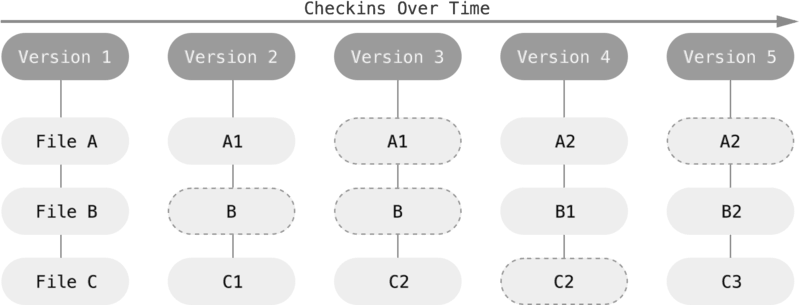
\includegraphics[width=\linewidth]{git-snapshots.png}
  \end{center}
  \caption{Зберігання даних у вигляді знімків станів}
  \label{img:git_snapshots}
\end{figure}

На перший погляд це може здатися затратним по об'єму пам'яті, який знадобиться для 
копіювання знімків станів. Але, по-перше,
Git проводить внутрішні оптимізації та не копіює знімки
файлів що не змінилися. Замість цього в репозиторії зберігаються малі за розміром посилання
на попередні знімки файлів. По-друге, хоча це і справді трохи збільшує розмір репозиторію,
на практиці, різниця майже непомітна адже звичайні текстові файли, які часто знаходяться
під контролем такої системи, займають дуже мало місця. По-третє, такі незначні недоліки
повністю нівелюються функціоналом, який подібна система може запропонувати.

Незважаючи на свій розподілений характер, всі операції в системі Git здійснюються локально,
без підключення до мережі, тому інформація з інших ком'ютерів, на яких відслідковується
такий самий репозиторій, не потрібна. Як наслідок, усі операції здійснюються практично
моментально. Що дуже контрастує із іншою системою Subversion, у якій вся інформація
зберігається на віддаленому сервері, і будь-яка зміна потребує оновлення на цьому
віддаленому сервері.

У системі Git для всіх даних, перед збереженням, зберігається так звана контрольна сума.
Це дає змогу забезпечити цілісність даних та високий рівень контролю над тим
вмістом, який потрапляє до репозиторію. Також, Git, як правило, тільки додає
інформацію, тому дуже складно зробити невідворотню дію. Якщо щось потрапило до
репозиторію, то це гарантовано можна буде відновити. Це дає можливість не боятися
за стан локальних файлів та експерементувати. Користувач модифікує файли у робочій папці,
які на цей момент мають статус ``такі, що не відслідковуються'' (unstaged). Система,
як зрозуміло із назви, не відслідковує зміни в таких файлах. Їх дуже просто видалити
і повернутися до стану файлів, які мають статус ``зафіксовані'' (commited).

Основною перевагою системи Git, серед багатьох інших, є система створення гілок, яка
дозволяє вести розробку паралельно і мати декілька версій проекту одночасно. Це унікальна
особливість Git, яка стала можливою завдяки згаданому раніше підходу збереження даних
у вигляді знімків станів (рис. \ref{img:git_snapshots}). Гілки у Git є дуже легковісними
вказівниками на контрольну суму зафіксованих файлів, тому операція створення гілки
відбувається миттєво. Переключання гілок ніяк не впливає на стан файлів репозиторія,
але змінює стан файлів у робочій папці. Потужна система гілок Git виводить розробку
програмного забезпечення на якісно новий рівень та сильно виділяє Git з-поміж аналогів
систем контролю версій.

Список функцій системи Git не обмежується переліченими вище, але у цій роботі 
використовувалися тільки згадані можливості.

\subsubsection{Інтернет хостинг GitHub}
Вихідний код програмного продукту цієї роботи розміщено на платформі GitHub.
Це найбільший хостинг Git репозиторіїв та, одночасно, майданчик для співробітництва
мільйонів розробників зі всього світу.

Оскільки Git є розподіленою системою, так зване ``джерело правди'' знаходиться у кожного,
хто має відповідний репозиторій на своєму комп'ютері. Але дуже зручно мати ``головний''
репозиторій, де синхронізуються всі зміни. І у разі втрати локальних даних, їх дуже просто
відновити.

На сайті GitHub зберігається точна копія локального репозиторія і відрізняєтся лише тим,
що там система Git виступає у якості сервера. На ньому не ведеться безпосередня розробка,
туди потрапляють дані із всіх клонованих репозиторіїв. А GitHub, в свою чергу, надає
можливість управління цим віддаленим репозиторієм через систему запитів на злиття
(pull request) та можливістю створити захищені гілки, в які напряму не можна нічого
зливати. Це можна буде зробити тільки після схвалення оглядачів. Тому будь-хто може
взяти участь у розробці проекту що зацікавив. Але в той самий час є запобіжники у
вигляді вищезгаданих механізмів, які не дозволяють зіпсувати чи якось нашкодити
проекту, шляхом написання неякісного коду, або такого, що не відповідає стандартам
відповідного проекту.


\subsection{Утиліти Universal Dependencies для обробки даних}


%-----------------------------------%


\newpage
\phantomsection
\addcontentsline{toc}{section}{ВИСНОВКИ}

\begin{center}
\textbf{\Large ВИСНОВКИ}
\end{center}